\documentclass{article} % Класс печатного документа

% для поддержки русского языка
\usepackage[T2A]{fontenc} % поддержка специальных русских символов
\usepackage[utf8]{inputenc} % Кодировка исходного текста - utf8
\usepackage[english,russian]{babel} % Поддержка языка - русского с английским
\usepackage{indentfirst} % Отступ в первом абзаце

\usepackage{graphicx} % Для вставки картинок
\usepackage{hyperref} % Для вставки гиперссылок
\usepackage{listings} % Для вставки кусков кода
\usepackage{float} % Для точного позиционирования картинок
\usepackage{amsmath} % Для отключения нумерации у указанных формул
\usepackage{listings} % Добавление листингов
\usepackage[justification=centering]{caption} % для центрирования подписи к таблице

\title{Отчёт 3\\
Определение необходимого числа компонент\\
метода главных компонент} % заголовок документа
\author{Свичкарев А.\,В.} % Автор документа
\date{\today} % Текущая дата

\begin{document} % Конец преамбулы, начало текста

\maketitle % Печатает заголовок, список авторов и дату

\section*{Задачи}
В таблице приведены данные по 32 экземплярам,
каждый из которых характеризуется 12 признаками.

На основе метода главных компонент найти количество главных компонент,
которого будет достаточно для описания экземпляров предложенной задачи.

\begin{table}[H]
\centering
\caption{Исходная таблица}
\begin{tabular}{|l|l|l|l|l|l|l|l|l|l|l|l|}
\hline
A1  & A2 & A3 & A4 & A5 & A6   & A7  & A8  & A9 & A10 & A11 & A12 \\ \hline
198 & 92 & -1 & 48 & 48 & 45   & 420 & 115 & -1 & 98  & -1  & 100 \\ \hline
184 & 84 & -1 & 44 & 33 & 33   & 350 & 102 & -1 & 92  & -1  & 130 \\ \hline
183 & 83 & -1 & 44 & 37 & 34   & 320 & 98  & -1 & 91  & -1  & 127 \\ \hline
182 & 80 & -1 & 42 & 35 & 30   & 398 & 65  & -1 & 85  & -1  & 140 \\ \hline
180 & 80 & -1 & 43 & 36 & 30   & 388 & 63  & -1 & 84  & -1  & 129 \\ \hline
183 & 81 & -1 & 42 & 37 & 35   & 345 & 45  & -1 & 90  & -1  & 105 \\ \hline
180 & 82 & -1 & 44 & 43 & 37   & 355 & 82  & -1 & 88  & -1  & 109 \\ \hline
180 & 81 & -1 & 44 & 46 & 42   & 362 & 90  & -1 & 86  & -1  & 113 \\ \hline
185 & 82 & -1 & 45 & 26 & 16   & 295 & 180 & -1 & 92  & 1   & 109 \\ \hline
187 & 84 & -1 & 46 & 27 & 16.5 & 299 & 178 & -1 & 95  & 1   & 119 \\ \hline
177 & 65 & -1 & 41 & 26 & 18   & 209 & 160 & -1 & 86  & 1   & 120 \\ \hline
180 & 72 & -1 & 43 & 33 & 19   & 236 & 175 & -1 & 85  & 1   & 115 \\ \hline
181 & 75 & -1 & 43 & 42 & 31   & 198 & 161 & -1 & 83  & 1   & 105 \\ \hline
176 & 68 & -1 & 42 & 50 & 36   & 195 & 177 & -1 & 82  & 1   & 96  \\ \hline
175 & 67 & 1  & 42 & 55 & 38   & 185 & 187 & -1 & 80  & 1   & 105 \\ \hline
178 & 75 & -1 & 42 & 30 & 24   & 203 & 208 & -1 & 81  & 1   & 118 \\ \hline
166 & 47 & -1 & 36 & 32 & 28   & 270 & 78  & 1  & 75  & -1  & 112 \\ \hline
170 & 60 & 1  & 38 & 23 & 20   & 312 & 99  & 1  & 81  & -1  & 110 \\ \hline
172 & 64 & 1  & 39 & 24 & 22   & 308 & 91  & 1  & 82  & -1  & 102 \\ \hline
169 & 51 & 1  & 36 & 24 & 23   & 250 & 89  & 1  & 78  & -1  & 98  \\ \hline
168 & 52 & 1  & 37 & 27 & 23.5 & 260 & 86  & 1  & 78  & -1  & 100 \\ \hline
157 & 47 & 1  & 36 & 32 & 32   & 235 & 92  & 1  & 70  & -1  & 127 \\ \hline
164 & 50 & 1  & 38 & 41 & 34   & 255 & 134 & 1  & 76  & -1  & 101 \\ \hline
162 & 49 & 1  & 37 & 40 & 34   & 265 & 124 & 1  & 75  & -1  & 108 \\ \hline
168 & 50 & 1  & 37 & 49 & 34   & 170 & 162 & 1  & 76  & 1   & 135 \\ \hline
166 & 49 & 1  & 36 & 21 & 14   & 150 & 245 & 1  & 75  & 1   & 123 \\ \hline
158 & 46 & 1  & 34 & 30 & 18   & 120 & 120 & 1  & 70  & 1   & 119 \\ \hline
163 & 50 & 1  & 36 & 18 & 11   & 143 & 136 & 1  & 75  & 1   & 102 \\ \hline
162 & 50 & 1  & 36 & 20 & 11.5 & 133 & 146 & 1  & 74  & 1   & 132 \\ \hline
165 & 51 & 1  & 36 & 36 & 26   & 121 & 129 & 1  & 76  & 1   & 126 \\ \hline
161 & 48 & 1  & 35 & 41 & 31.5 & 116 & 196 & 1  & 75  & 1   & 120 \\ \hline
160 & 48 & 1  & 35 & 40 & 31   & 118 & 198 & 1  & 74  & 1   & 129 \\ \hline
\end{tabular}
\end{table}

\clearpage
\section*{Выполнение}
\begin{figure}[H]
    \centering
    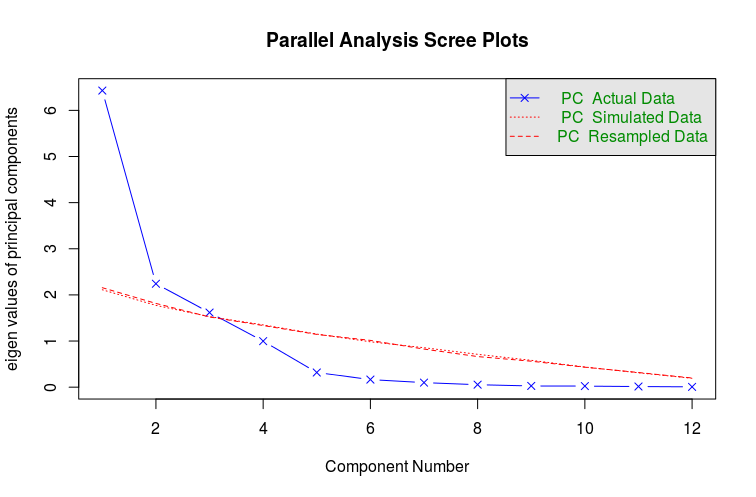
\includegraphics[width=\textwidth]{scree}
    \caption{Диаграмма каменистой осыпи с параллельным анализом}
\end{figure}

Это графическое изображение результатов теста собственных значений
(обозначены отрезками и крестиками) и усредненных собственных
значений, полученных из 100 случайных таблиц данных (пунктир).

Согласно критерию Кайзера-Харриса (Kaiser-Harris),
следует использовать компоненты, у которых собственные значения
превышают единицу.

Если собственное значение, основанное на реальных данных,
выше, чем соответствующие усредненные собственные значения для
набора случайных матриц данных, тогда такая компонента используется.
Подобный подход называется параллельным анализом.

Таким образом имеет смысл выделить 2 главных компоненты
(можно и 3, но третья почти на одном уровне с симулированными данными).

Результат выделения двух главных компонент:

\begin{lstlisting}
Principal Components Analysis
Call: principal(r = data, nfactors = 2)
Standardized loadings (pattern matrix) based upon correlation matrix
              PC1   PC2    h2    u2 com
Attribute1   0.96  0.17 0.947 0.053 1.1
Attribute2   0.96  0.20 0.962 0.038 1.1
Attribute3  -0.88 -0.11 0.784 0.216 1.0
Attribute4   0.97  0.15 0.968 0.032 1.0
Attribute5   0.30  0.22 0.140 0.860 1.8
Attribute6   0.29  0.58 0.418 0.582 1.5
Attribute7   0.59  0.73 0.891 0.109 1.9
Attribute8   0.02 -0.89 0.788 0.212 1.0
Attribute9  -0.96 -0.01 0.916 0.084 1.0
Attribute10  0.92  0.19 0.884 0.116 1.1
Attribute11 -0.01 -0.96 0.928 0.072 1.0
Attribute12 -0.04 -0.21 0.046 0.954 1.1

                       PC1  PC2
SS loadings           5.85 2.82
Proportion Var        0.49 0.24
Cumulative Var        0.49 0.72
Proportion Explained  0.67 0.33
Cumulative Proportion 0.67 1.00

Mean item complexity =  1.2
Test of the hypothesis that 2 components are sufficient.

The root mean square of the residuals (RMSR) is  0.11 
 with the empirical chi square  52.27  with prob <  0.16 

Fit based upon off diagonal values = 0.96
\end{lstlisting}

Имеет смысл обратить внимание на строку Proportion var и Cumulative Var,
которые показывают сколько процентов дисперсии признаков
учитывает каждая компонента.
Первая компонента учитывает 49\% дисперсии всех признаков,
а вторая компонента – 24\%.
Вместе эти две компоненты объясняют 72\% общей дисперсии.

Можно попробовать выделить 3 компоненты:
\begin{lstlisting}
Proportion Var        0.48 0.21 0.16
Cumulative Var        0.48 0.70 0.86
\end{lstlisting}
тогда в общем учитывается 86\% дисперсии признаков,
что немного лучше.

При учёте 4 компонент --- 94\%.

Однако, компоненты с собственными значениями меньше единицы (4-ая компонента)
объясняют меньше дисперсии, чем содержится в одной исходной переменной.

\section*{Вывод}
Для данной выборки разумно выделить 2-3 главных компоненты.

\section*{Исходный код}
Исходный код прилагается.

\end{document} % Конец документа
